This section presents the experimental study carried out to validate the performance of \DEEDM{}.
%
Specifically, we show that by explicitly controlling the diversity in \DE{}, results of state-of-the-art algorithms
are improved further.
%
Particularly, the benchmarks of \CEC{} 2016 and \CEC{} 2017 are considered.
%
Each one of them is composed of thirty different problems, meaning that the validation is performed with a set of large and diverse
functions.
%
The kind of problems of each benchmark is divided in uni-modal, 
simple multi-modal, hybrid and composition functions.
%
Table \ref{tab:category} shows the problems belonging to each category for the \CEC{} 2016 and \CEC{} 2017 benchmarks.
%
%Principally,  in the real-world optimization problems, different sub-components of the variables may have different properties.
%
In the hybrid functions, the variables are randomly divided into some sub-components and each one is related to basic functions.
%
In the same line, the composition functions merge the properties of several sub-functions and maintains continuity around each local optima.
%
Also the local optima which has the smallest bias value is the global optimum.
%
The search space is bounded by the range $\Omega = \prod_{j=1}^D[-100, 100]^D$.

\begin{table}[t]
\centering
\begin{tabular}{|c|c|c|}
\hline
\textbf{Type Function} & \textbf{CEC 2016} & \textbf{CEC 2017} \\ \hline
\textbf{Uni-modal} & $f_1$ - $f_3$ & $f_1$ - $f_3$ \\ \hline
\textbf{Simple multi-modal} & $f_4$ - $f_{16}$ & $f_4$ - $f_{10}$ \\ \hline
\textbf{Hybrid (multi-modal)} & $f_{17}$ - $f_{22}$ & $f_{11}$ - $f_{20}$ \\ \hline
\textbf{Composition (multi-modal)} & $f_{23}$ - $f_{30}$ & $f_{21}$ - $f_{30}$ \\ \hline
\end{tabular}
\caption{Problems grouped by properties for the \CEC{} 2016 and \CEC{} 2017 benchmarks}\label{tab:category}
\end{table}
%
The experimental validation takes into account the algorithms that attained the first places of each year competition,
as well as the standard \DE{}.
%
Additionally, comparisons against other diversity-based schemes are included.
%
The algorithms considered from the \CEC{} 2016 are UMOEAs-II \cite{elsayed2016testing} and L-SHADE-EpSin \cite{awad2016ensemble}, 
which achieved the first and second places respectively.
%
Similarly, the top algorithms from \CEC{} 2017 are taken into account, i.e. EBOwithCMAR~\cite{kumar2017improving} 
and jSO~\cite{brest2017single}.
%
%It is interesting to remark that EBOwithCMAR is considered as an improvement of the UMOEAs-II.
%
%Additionally, jSO and L-SHADE-EpSin belong to the SHADE's family.
%
Following the recommendations given in~\cite{molina2017analysis}, all these algorithms are tested with both benchmarks.

Given that the optimizers taken into account are stochastic algorithms, each execution was repeated 51 times with different seeds.
%
In every case, the stopping criterion was set to $25 \times 10^6$ functions evaluations.
%
In addition, problems were configured by setting $D = 10$. 
%
The validation follows the guidelines of \CEC{} benchmark competitions and the statistical tests proposed in~\cite{Joel:StatisticalTest} are also included.
%
%The first, considers a composed score between the mean of difference error and the rank of the algorithms.
%
%The second, follows a statistical scheme, which applies pair-comparisons based on the distribution of the error between the algorithms.
%
Note that, as it is usual in these competitions, when the gap between the values of the best solution found and the optimal solution is $10^{-8}$ or smaller, 
the error is treated as $0$.
%
%The minimal tolerance to consider a determined problem solved is $1e-8$, hence if the difference of the optimal obtained and the true optinal is below this tolerance then the error is zero.
%
The parameterization indicated by the authors was used in every algorithm and it is as follows:
\begin{itemize}
\item \textbf{EBOwithCMAR}: For EBO, the maximum population size of $S_1 = 18D$, minimum population size of $S_1 = 4$, maximum population size of $S_2 = 146.8D$, minimum population size of $S_2 = 10$, historical memory size H=$6$. For CMAR Population size $S_3 = 4 + 3log(D)$, $\sigma=0.3$, CS = $50$, probability of local search $pl = 0.1$ and $cfe_{ls} = 0.4* FE_{max}$.
\item \textbf{UMOEAs-II}: For MODE, maximum population size of $S_1 = 18D$, minimum population size of $S_1 = 4$, size memory H=$6$. For CMA-ES Population size $S_2 = 4 + \lfloor 3log(D) \rfloor$, $\mu=\frac{N}{2}$, $\sigma=0.3$, CS = $50$. For local search, $cfe_{ls} = 0.2 * FE_{max}$.
\item \textbf{jSO}: Maximum population size = $25log(D)\sqrt{D}$, historical memory size H= $5$, initial mutation memory $M_F = 0.5$, initial probability memory $M_{CR} = 0.8$, minimum population size = $4$, initial p-best = $0.25*N$, final p-best = $2$.
\item \textbf{L-SHADE-EpSin}: Maximum population size = $25log(D)\sqrt{D}$, historical memory size H= $5$, initial mutation memory $M_F = 0.5$, initial probability memory $M_{CR} = 0.5$, initial memory frequency $\mu_F = 0.5$, minimum population size = $4$, initial p-best = $0.25*N$, final p-best = $2$, generations of local search $G_{LS}=250$.
\item \textbf{ DE-EDM}: $D_I = 0.3$, population size = $250$, CR $\sim Normal( \{0.2, 0.9\}, 0.1)$, F $\sim Cauchy(0.5, 0.5*nfes/max_{nfes})$.
\item \textbf{ Standard-DE}: population size = $250$ (operators as \DEEDM{}), CR $\sim Normal( \{0.2, 0.9\}, 0.1)$, F $\sim Cauchy(0.5, 0.5*nfes/max_{nfes})$.
\end{itemize}
%

Our experimental analyses is based on the error, i.e. the difference between the optimal solution and the best obtained solution.
%
In order to statistically compare the results, a similar guideline than the one proposed in~\cite{Joel:StatisticalTest} was used. 
%
First a Shapiro-Wilk test was performed to check whatever or not the values of the results followed a Gaussian distribution. 
%
If, so, the Levene test was used to check for the homogeneity of the variances. 
%
If samples had equal variance, an ANOVA test was done; if not, a Welch test was performed. 
%
For non-Gaussian distributions, the non parametric Kruskal-Wallis test was used to test whether samples are drawn from the same distribution. 
%
An algorithm $X$ is said to win algorithm $Y$ when the differences between them are statistically significant, and the mean and median error obtained by $X$ are lower 
than the mean and median achieved by $Y$.

Tables \ref{tab:Summary_CEC2016} and \ref{tab:Summary_CEC2017} offer a summary of the results obtained for \CEC{} 2016 and \CEC{} 2017, respectively.
%
The column tagged with ``Always Solved'' shows the number of functions where a zero error was obtained in the 51 runs.
%
Additionally, column tagged with ``At least one time solved'' shows the number of functions that were solved at least in one run.
%
Practically all functions (28 of them) of the \CEC{} 2017 benchmark were solved with \DEEDM{} at least one time.
%
Additionally, 21 functions of the \CEC{} 2016 were also solved.
%
This contrasts with the results obtained by state-of-the-art algorithms.
%
They were able to reach optimal values in significantly less functions.
%
In order to confirm the superiority of \DEEDM{}, the pair-wise statistical tests already described were used.
%
The column tagged with the symbol $\uparrow$ shows the number of cases where the superiority of each method could be confirmed, whereas
the column tagged with the symbol $\downarrow$ counts the number of cases where the method was inferior.
%
Finally, the number comparisons with not significant differences are shown in the column tagged with the symbol $\longleftrightarrow$.
%
The results of the statistical tests show that \DEEDM{} attained the best results in both years.
%
The number of victories in \CEC{} 2016 and \CEC{} 2017 were $77$ and $88$, whereas 
the number of losses were $25$ and $6$, respectively.
%
\DEEDM{} is the approach with the largest number of victories and lowest number of losses in both benchmarks, confirming the superiority
of the proposal.
%Additionally, the last place attained in both years was by the L-SHADE-Epsilon with $20$ wins in 2016 and $7$ wins in 2017.
%
%
The last column --- tagged with ``Score'' --- considers the official score of \CEC{}'s competitions.
%
Particularly, the raking of the algorithms is attained by taking into account the two scores defined in Eq. (\ref{eqn:total_scores}).
%
Then, the final score is calculated as the sum $Score = Score_1 + Score_2$.
%
In Eq.~(\ref{eqn:total_scores}), the $SE$ of an algorithm is the sum of the mean error values obtained in the $30$ benchmark functions, i.e. 
$SE = \sum_{i=1}^{30} error\_f_i$ .
%
Then, $SE_{min}$ is the minimal $SE$ from all the algorithms. 
%
In order to calculate $SR$ and $SR_{min}$, algorithms are sorted in each function in base of the attained mean error.
%
Then, a rank is assigned to each algorithm in base of such an ordering.
%
Finally, the $SR$ of a method is the sum of the ranks obtained for each function and $SR_{min}$ is the minimal $SR$ from all the algorithms.

% Please add the following required packages to your document preamble:
% \usepackage{multirow}
\begin{table}[t]
%\begin{scriptsize}
\centering
\caption{Summary results - \CEC{} 2016}
\label{tab:Summary_CEC2016}
\begin{tabular}{|c|c|c|c|c|c|c|}
\hline
\multirow{2}{*}{\textbf{Algorithm}} & \multirow{2}{*}{\textbf{\begin{tabular}[c]{@{}c@{}}Always \\ solved\end{tabular}}} & \multirow{2}{*}{\textbf{\begin{tabular}[c]{@{}c@{}}At least one\\ time solved\end{tabular}}} & \multicolumn{3}{c|}{\textbf{Statistical Tests}} & \multirow{2}{*}{\textbf{Score}} \\ \cline{4-6}
 &  &  & $\uparrow$ & $\downarrow$ & $\longleftrightarrow $ &  \\ \hline
\textbf{DE-EDM} & 13 & 21 & 77 & 25 & 48 & 100.00 \\ \hline
\textbf{UMOEAs-II} & 9 & 14 & 51 & 31 & 68 & 62.45 \\ \hline
\textbf{Standard-DE} & 11 & 19 & 50 & 46 & 54 & 56.29 \\ \hline
\textbf{jSO} & 9 & 17 & 47 & 51 & 52 & 55.43 \\ \hline
\textbf{EBOwithCMAR} & 8 & 14 & 35 & 56 & 59 & 50.28 \\ \hline
\textbf{L-SHADE-Epsilon} & 7 & 13 & 20 & 71 & 59 & 50.12 \\ \hline
\end{tabular}
%\end{scriptsize}
\end{table}

% Please add the following required packages to your document preamble:
% \usepackage{multirow}
\begin{table}[t]
%\begin{scriptsize}
\centering
\caption{Summary results - \CEC{} 2017}
\label{tab:Summary_CEC2017}
\begin{tabular}{|c|c|c|c|c|c|c|}
\hline
\multirow{2}{*}{\textbf{Algorithm}} & \multirow{2}{*}{\textbf{\begin{tabular}[c]{@{}c@{}}Always \\ solved\end{tabular}}} & \multirow{2}{*}{\textbf{\begin{tabular}[c]{@{}c@{}}At least one\\ time solved\end{tabular}}} & \multicolumn{3}{c|}{\textbf{Statistical Tests}} & \multirow{2}{*}{\textbf{Score}} \\ \cline{4-6}
 &  &  & $\uparrow$ & $\downarrow$ & $\longleftrightarrow $ &  \\ \hline
\textbf{DE-EDM} & 21 & 28 & 88 & 6 & 56 & 100.00 \\ \hline
\textbf{Standard-DE} & 12 & 21 & 56 & 29 & 65 & 42.91 \\ \hline
\textbf{EBOwithCMAR} & 9 & 18 & 34 & 46 & 70 & 37.14 \\ \hline
\textbf{L-SHADE-Epsilon} & 8 & 19 & 7 & 81 & 62 & 32.78 \\ \hline
\textbf{jSO} & 8 & 15 & 29 & 55 & 66 & 29.30 \\ \hline
\textbf{UMOEAs-II} & 11 & 15 & 43 & 40 & 67 & 26.89 \\ \hline
\end{tabular}
%\end{scriptsize}
\end{table}

\begin{equation}\label{eqn:total_scores}
\begin{split}
Score_1 &= \left (1 - \frac{SE - SE_{min}}{SE} \right) \times 50, \\
Score_2 &= \left  (1 - \frac{SR - SR_{min}}{SR} \right ) \times 50, \\
\end{split}
\end{equation}

Note that in base of this definition, the best attainable score is $100$.
%
This happens when a given approach obtains both $SR_{min}$ and $SE_{min}$.
%
\DEEDM{} attained the best attainable score in both years, which confirms its clear superiority when compared both with state-of-the-art and standard \DE{}.
%
In these long-term executions, standard \DE{} attained the third and second places in the problems of 
the \CEC{} 2016 and \CEC{} 2017, respectively.
%
This means that the performance of the state-of-the-art algorithms is not so impressive in long-term executions.
%
%Specifically, although that in \CEC{} 2017 the L-SHADE-Epsilon algorithm got the lowest number of wins in the statistical test it showed a competitive score.
%
%This might occurs since that the statistical scores considers both mean and median errors.
%
%Morever, the score considers a rank and mean based on the error.
%

%TODO: Poner Dado que nuestra novedad está en el control de la diversidad, para comprender mejor el comportamiento de la propuesta...

Since our proposal is based on the explicit control of diversity, Fig. \ref{fig:diversity} shows the evolution of the mean of the diversity calculated
as the mean distance to the closest vector with the aim of better understanding its behavior.
%
Particularly, functions $f_1$ and $f_{30}$ were selected for this analysis because they have quite different features (easy uni-modal vs. complex multi-modal).
%
The left side shows the diversity of the Elite population.
%
It is remarkable that, while there are no direct constraints in the Elite population related to diversity, 
the diversity is implicitly maintained.
%
The right side shows the diversity of the target vectors.
%
As expected, diversity decreases in a gradual way and a degree of diversity is maintained until the $90\%$ of the total function evaluations is reached.

\begin{figure}[t]
\centering
\begin{tabular}{cc}
   \includegraphics[scale=0.23, angle=-90]{Diversity_Elite.eps} 
   \includegraphics[scale=0.23, angle=-90]{Diversity_Target.eps} 
\end{tabular}
\caption{Mean distance to the closest vector of the 51 executions with the problems $f_1$ and $f_{30}$ (\CEC{} 2016 and \CEC{} 2017). The initial distance factor considered corresponds to $D_I=0.3$}
\label{fig:diversity}
\end{figure}



Finally, in order to provide comparable results of our proposal, Tables~\ref{tab:Results_CEC2016} and~\ref{tab:Results_CEC2017} report the best, worst, median, 
mean, standard deviation and success rate for both benchmarks.
%
These tables show that all the uni-modal problems were solved by our proposal.
%
Additionally, several simple and even some of the most complex multi-modal functions were optimally solved.
%
In fact, several complex functions that had never been solved by state-of-the-art could be solved by \DEEDM{}.
%
\begin{table}[t]
\begin{scriptsize}
\centering
\caption{Results for \DEEDM{} in the \CEC{} 2016 problems}
\label{tab:Results_CEC2016}
%\resizebox{\textwidth}{!}{%
\begin{tabular}{|c|c|c|c|c|c|c|}
\hline
 & \textbf{Best} & \textbf{Worst} & \textbf{Median} & \textbf{Mean} & \textbf{Std.} & \textbf{Succ. Rate} \\ \hline
$f_1$ & 0.00E+00 & 0.00E+00 & 0.00E+00 & 0.00E+00 & 0.00E+00 & 1.00E+00 \\ \hline
$f_2$ & 0.00E+00 & 0.00E+00 & 0.00E+00 & 0.00E+00 & 0.00E+00 & 1.00E+00 \\ \hline
$f_3$ & 0.00E+00 & 0.00E+00 & 0.00E+00 & 0.00E+00 & 0.00E+00 & 1.00E+00 \\ \hline
$f_4$ & 0.00E+00 & 0.00E+00 & 0.00E+00 & 0.00E+00 & 0.00E+00 & 1.00E+00 \\ \hline
$f_5$ & 0.00E+00 & 0.00E+00 & 0.00E+00 & 0.00E+00 & 0.00E+00 & 1.00E+00 \\ \hline
$f_6$ & 0.00E+00 & 3.60E-02 & 4.00E-03 & 7.39E-03 & 1.15E-02 & 3.92E-01 \\ \hline
$f_7$ & 2.00E-02 & 1.02E-01 & 5.90E-02 & 5.77E-02 & 4.93E-02 & 0.00E+00 \\ \hline
$f_8$ & 0.00E+00 & 0.00E+00 & 0.00E+00 & 0.00E+00 & 0.00E+00 & 1.00E+00 \\ \hline
$f_9$ & 0.00E+00 & 0.00E+00 & 0.00E+00 & 0.00E+00 & 0.00E+00 & 1.00E+00 \\ \hline
$f_{10}$ & 0.00E+00 & 0.00E+00 & 0.00E+00 & 0.00E+00 & 0.00E+00 & 1.00E+00 \\ \hline
$f_{11}$ & 0.00E+00 & 6.00E-02 & 0.00E+00 & 5.88E-03 & 1.90E-02 & 9.02E-01 \\ \hline
$f_{12}$ & 0.00E+00 & 0.00E+00 & 0.00E+00 & 0.00E+00 & 0.00E+00 & 1.00E+00 \\ \hline
$f_{13}$ & 1.00E-02 & 8.00E-02 & 5.00E-02 & 4.67E-02 & 2.60E-02 & 0.00E+00 \\ \hline
$f_{14}$ & 1.00E-02 & 5.00E-02 & 3.00E-02 & 2.82E-02 & 2.13E-02 & 0.00E+00 \\ \hline
$f_{15}$ & 0.00E+00 & 4.70E-01 & 2.20E-01 & 1.99E-01 & 1.55E-01 & 1.96E-02 \\ \hline
$f_{16}$ & 4.00E-02 & 1.50E-01 & 8.00E-02 & 8.47E-02 & 4.96E-02 & 0.00E+00 \\ \hline
$f_{17}$ & 0.00E+00 & 0.00E+00 & 0.00E+00 & 0.00E+00 & 0.00E+00 & 1.00E+00 \\ \hline
$f_{18}$ & 0.00E+00 & 2.00E-02 & 1.00E-02 & 7.65E-03 & 6.32E-03 & 3.14E-01 \\ \hline
$f_{19}$ & 0.00E+00 & 0.00E+00 & 0.00E+00 & 0.00E+00 & 0.00E+00 & 1.00E+00 \\ \hline
$f_{20}$ & 0.00E+00 & 0.00E+00 & 0.00E+00 & 0.00E+00 & 0.00E+00 & 1.00E+00 \\ \hline
$f_{21}$ & 0.00E+00 & 0.00E+00 & 0.00E+00 & 0.00E+00 & 0.00E+00 & 1.00E+00 \\ \hline
$f_{22}$ & 0.00E+00 & 3.00E-02 & 0.00E+00 & 3.73E-03 & 2.76E-02 & 7.65E-01 \\ \hline
$f_{23}$ & 0.00E+00 & 1.00E+02 & 0.00E+00 & 2.55E+01 & 5.10E+01 & 7.45E-01 \\ \hline
$f_{24}$ & 0.00E+00 & 6.90E-01 & 0.00E+00 & 2.61E-02 & 1.33E-01 & 9.61E-01 \\ \hline
$f_{25}$ & 1.00E+02 & 1.00E+02 & 1.00E+02 & 1.00E+02 & 0.00E+00 & 0.00E+00 \\ \hline
$f_{26}$ & 8.00E-02 & 1.00E+02 & 5.29E+01 & 5.20E+01 & 3.19E+01 & 0.00E+00 \\ \hline
$f_{27}$ & 2.50E-01 & 9.10E-01 & 5.40E-01 & 5.60E-01 & 2.92E-01 & 0.00E+00 \\ \hline
$f_{28}$ & 0.00E+00 & 3.57E+02 & 3.43E+02 & 2.76E+02 & 1.60E+02 & 1.96E-01 \\ \hline
$f_{29}$ & 1.00E+02 & 1.00E+02 & 1.00E+02 & 1.00E+02 & 0.00E+00 & 0.00E+00 \\ \hline
$f_{30}$ & 1.84E+02 & 1.84E+02 & 1.84E+02 & 1.84E+02 & 3.25E-02 & 0.00E+00 \\ \hline
\end{tabular}%
%}
\end{scriptsize}
\end{table}

\begin{table}[t]
\begin{scriptsize}
\centering
\caption{Results for \DEEDM{} in the \CEC{} 2017 problems}
\label{tab:Results_CEC2017}
%\resizebox{\textwidth}{!}{%
\begin{tabular}{|c|c|c|c|c|c|c|}
\hline
 & \textbf{Best} & \textbf{Worst} & \textbf{Median} & \textbf{Mean} & \textbf{Std.} & \textbf{Succ. Ratio} \\ \hline
$f_1$ & 0.00E+00 & 0.00E+00 & 0.00E+00 & 0.00E+00 & 0.00E+00 & 1.00E+00 \\ \hline
$f_2$ & 0.00E+00 & 0.00E+00 & 0.00E+00 & 0.00E+00 & 0.00E+00 & 1.00E+00 \\ \hline
$f_3$ & 0.00E+00 & 0.00E+00 & 0.00E+00 & 0.00E+00 & 0.00E+00 & 1.00E+00 \\ \hline
$f_4$ & 0.00E+00 & 0.00E+00 & 0.00E+00 & 0.00E+00 & 0.00E+00 & 1.00E+00 \\ \hline
$f_5$ & 0.00E+00 & 0.00E+00 & 0.00E+00 & 0.00E+00 & 0.00E+00 & 1.00E+00 \\ \hline
$f_6$ & 0.00E+00 & 0.00E+00 & 0.00E+00 & 0.00E+00 & 0.00E+00 & 1.00E+00 \\ \hline
$f_7$ & 0.00E+00 & 0.00E+00 & 0.00E+00 & 0.00E+00 & 0.00E+00 & 1.00E+00 \\ \hline
$f_8$ & 0.00E+00 & 0.00E+00 & 0.00E+00 & 0.00E+00 & 0.00E+00 & 1.00E+00 \\ \hline
$f_9$ & 0.00E+00 & 0.00E+00 & 0.00E+00 & 0.00E+00 & 0.00E+00 & 1.00E+00 \\ \hline
$f_{10}$ & 0.00E+00 & 1.20E-01 & 0.00E+00 & 1.65E-02 & 3.39E-02 & 7.45E-01 \\ \hline
$f_{11}$ & 0.00E+00 & 0.00E+00 & 0.00E+00 & 0.00E+00 & 0.00E+00 & 1.00E+00 \\ \hline
$f_{12}$ & 0.00E+00 & 2.20E-01 & 0.00E+00 & 6.37E-02 & 1.76E-01 & 6.67E-01 \\ \hline
$f_{13}$ & 0.00E+00 & 0.00E+00 & 0.00E+00 & 0.00E+00 & 0.00E+00 & 1.00E+00 \\ \hline
$f_{14}$ & 0.00E+00 & 0.00E+00 & 0.00E+00 & 0.00E+00 & 0.00E+00 & 1.00E+00 \\ \hline
$f_{15}$ & 0.00E+00 & 0.00E+00 & 0.00E+00 & 0.00E+00 & 0.00E+00 & 1.00E+00 \\ \hline
$f_{16}$ & 0.00E+00 & 2.10E-01 & 0.00E+00 & 2.47E-02 & 7.27E-02 & 8.82E-01 \\ \hline
$f_{17}$ & 0.00E+00 & 0.00E+00 & 0.00E+00 & 0.00E+00 & 0.00E+00 & 1.00E+00 \\ \hline
$f_{18}$ & 0.00E+00 & 1.00E-02 & 0.00E+00 & 1.96E-03 & 4.47E-03 & 8.04E-01 \\ \hline
$f_{19}$ & 0.00E+00 & 0.00E+00 & 0.00E+00 & 0.00E+00 & 0.00E+00 & 1.00E+00 \\ \hline
$f_{20}$ & 0.00E+00 & 0.00E+00 & 0.00E+00 & 0.00E+00 & 0.00E+00 & 1.00E+00 \\ \hline
$f_{21}$ & 0.00E+00 & 0.00E+00 & 0.00E+00 & 0.00E+00 & 0.00E+00 & 1.00E+00 \\ \hline
$f_{22}$ & 0.00E+00 & 0.00E+00 & 0.00E+00 & 0.00E+00 & 0.00E+00 & 1.00E+00 \\ \hline
$f_{23}$ & 0.00E+00 & 3.00E+02 & 0.00E+00 & 3.49E+01 & 1.03E+02 & 8.82E-01 \\ \hline
$f_{24}$ & 0.00E+00 & 0.00E+00 & 0.00E+00 & 0.00E+00 & 0.00E+00 & 1.00E+00 \\ \hline
$f_{25}$ & 0.00E+00 & 1.00E+02 & 0.00E+00 & 3.92E+00 & 2.00E+01 & 9.61E-01 \\ \hline
$f_{26}$ & 0.00E+00 & 0.00E+00 & 0.00E+00 & 0.00E+00 & 0.00E+00 & 1.00E+00 \\ \hline
$f_{27}$ & 0.00E+00 & 3.87E+02 & 3.87E+02 & 2.05E+02 & 2.68E+02 & 1.96E-02 \\ \hline
$f_{28}$ & 0.00E+00 & 0.00E+00 & 0.00E+00 & 0.00E+00 & 0.00E+00 & 1.00E+00 \\ \hline
$f_{29}$ & 1.45E+02 & 2.26E+02 & 2.18E+02 & 1.99E+02 & 4.21E+01 & 0.00E+00 \\ \hline
$f_{30}$ & 3.95E+02 & 3.95E+02 & 3.95E+02 & 3.95E+02 & 2.10E-01 & 0.00E+00 \\ \hline
\end{tabular}%
%}
\end{scriptsize}
\end{table}

\begin{figure}[t]
\centering
  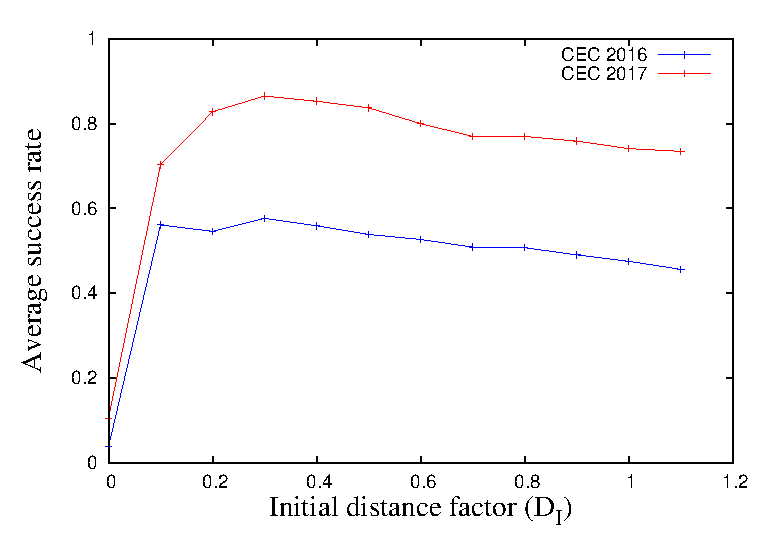
\includegraphics[scale=0.6]{Tuning_CEC.eps}
\caption{Mean success rate for different $D_I$ in the \CEC{} 2016 and \CEC{} 2017 benchmarks with a population size equal to $250$ and $25 \times 10^6$ function evaluations}
\label{fig:one}
\end{figure}

\subsection{Comparison of Diversity Replacement-Based Schemes}
%\subsection{Validation Against Diversity Replacement-Based Schemes}

In order to better validate the advantages provided by the replacement phase proposed in this paper, a meaningful comparison against two additional diversity replacement-based strategies were developed.
%
Particularly, the replacement-based methods taken into consideration are the \textit{Restricted Tournament Selection} (\RTS{}) 
and the \textit{Hybrid Genetic Search with Adaptive Diversity Control} (\HGSADC{}).
%
These replacement-based strategies were incorporated to the standard \DE{} framework.
% previously explained.
% using the same operators, i.e. mutation, 
%crossover and selection than in \DEEDM{}.
%
The three variants were executed with the same parameterization.
%
Note that both \RTS{} and \HGSADC{} require additional parameters.
%
Based on several analyses, the \RTS{} was executed with a sample size $CF=25$, differently the \HGSADC{} was considered with $N_{Close} = 1$,
and $N_{Elite}=8$.
%
The remaining configuration follows the same parameterization previously defined.
%
Tables \ref{tab:Summary_CEC2016_Replacement} and \ref{tab:Summary_CEC2017_Replacement} summarize the results attained
for both years with the same meaning that in the previous experiment.
%
Again, \DEEDM{} attained the best results in both years, also the second place was attained by \HGSADC{}.
%
It is clear that \DEEDM{} attained a significantly higher $Score$ than the remaining diversity-based methods.
%
Note that the main difference among our proposal in constrast to the schemes \RTS{} and \HGSADC{} is that they provide modifications
with the aim of delaying convergence.
%
However, this is performed in an indirect way, meaning that premature convergence might not always be avoided, so 
the process might search for a long period in just a few sub-optimal regions.
%
Second, while these methods have been quite successful in comparison to Evolutionary Algorithms with a high selection pressure,
\DE{} already incorporates a replacement strategy that follows some of the principles of crowding, 
thus there are not clear advantages of being incorporated in \DE{}.

%so the benefits of incorporating them in \DE{} seems to be much more reduced.
%
Therefore, the stopping criteria should be taken into account to avoid the premature convergence, particularly in long-term executions.

%taking into account the stopping criteria to explicitly avoid premature convergence, as it is done in our proposal, is quite important for the proper performance of long-term executions.


% Please add the following required packages to your document preamble:
% \usepackage{multirow}
\begin{table}[t]
\centering
\caption{Summary of the replacement algorithms - \CEC{} 2016}
\label{tab:Summary_CEC2016_Replacement}
\begin{tabular}{|c|c|c|c|c|c|c|}
\hline
\multirow{2}{*}{\textbf{Algorithm}} & \multirow{2}{*}{\textbf{\begin{tabular}[c]{@{}c@{}}Always \\ solved\end{tabular}}} & \multirow{2}{*}{\textbf{\begin{tabular}[c]{@{}c@{}}At least one\\ time solved\end{tabular}}} & \multicolumn{3}{c|}{\textbf{Statistical Tests}} & \multirow{2}{*}{\textbf{Score}} \\ \cline{4-6}
%\multirow{2}{*}{\textbf{Algorithm}} & \multirow{2}{*}{\textbf{Always solved}} & \multirow{2}{*}{\textbf{At least one time solved}} & \multicolumn{3}{c|}{\textbf{Statistical Tests}} & \multirow{2}{*}{\textbf{Score}} \\ \cline{4-6}
 &  &  & $\uparrow$ & $\downarrow$ & $\longleftrightarrow $ &  \\ \hline
\textbf{DE-EDM} & 13 & 21 & 51 & 1 & 8 & 100.00 \\ \hline
\textbf{RTS} & 2 & 7 & 3 & 47 & 10 & 19.74 \\ \hline
\textbf{HGSADC} & 3 & 15 & 21 & 27 & 12 & 44.12 \\ \hline
\end{tabular}
\end{table}


% Please add the following required packages to your document preamble:
% \usepackage{multirow}
\begin{table}[t]
\centering
\caption{Summary of the replacement algorithms - \CEC{} 2017}
\label{tab:Summary_CEC2017_Replacement}
\begin{tabular}{|c|c|c|c|c|c|c|}
\hline
\multirow{2}{*}{\textbf{Algorithm}} & \multirow{2}{*}{\textbf{\begin{tabular}[c]{@{}c@{}}Always \\ solved\end{tabular}}} & \multirow{2}{*}{\textbf{\begin{tabular}[c]{@{}c@{}}At least one\\ time solved\end{tabular}}} & \multicolumn{3}{c|}{\textbf{Statistical Tests}} & \multirow{2}{*}{\textbf{Score}} \\ \cline{4-6}
%\multirow{2}{*}{\textbf{Algorithm}} & \multirow{2}{*}{\textbf{Always solved}} & \multirow{2}{*}{\textbf{At least one time solved}} & \multicolumn{3}{c|}{\textbf{Statistical Tests}} & \multirow{2}{*}{\textbf{Score}} \\ \cline{4-6}
 &  &  & $\uparrow$ & $\downarrow$ & $\longleftrightarrow $ &  \\ \hline
\textbf{DE-EDM} & 21 & 28 & 49 & 0 & 11 & 100.00 \\ \hline
\textbf{RTS} & 4 & 12 & 2 & 49 & 9 & 30.91 \\ \hline
\textbf{HGSADC} & 6 & 18 & 23 & 25 & 12 & 40.86 \\ \hline
\end{tabular}
\end{table}


\subsection{Empirical Analyses of the Initial Distance Factor}

In our proposal the diversity is explicitly promoted and the total amount of diversity maintained in the population 
depends on the initial distance factor $D_I$.
%
Therefore, the effect of this parameter on the quality is analyzed in this section.
%
Particularly, the same scheme previously mentioned was taken into account.
%Particularly, the same scheme taken into accoun in the previous analyses was taken into account.
%
However, several initial distance factors were considered ($D_I = \{0.0, 0.1, 0.2, 0.3, 0.4, 0.5, 0.6, 0.7, 0.8, 0.9, 1.0, 1.1 \}$).


Fig. \ref{fig:one} shows the mean success rate attained for both benchmarks when considering different $D_I$ values.
%
The most relevant conclusions are:
\begin{itemize}
\item If diversity is not promoted ($D_I = 0.0 $) there is an important degradation in the performance. 
\item The performance is quite robust in the sense that a large range of $D_I$ values provide good enough results. For instance, values
in the range $[0.2, 0.6]$ provide high-quality solutions.
\item To a certain extent, if the initial distance factor ($D_I$) is very large (values larger than $0.6$), the quality of solutions is affected.% Therefore, as $D_I$ is increases the quality of solutions is gradually decreased.
%	This decrease of quality is gradual, i.e. as $D_I$ increases the quality slowly decreases.
\end{itemize}

To summarize, \DEEDM{} incorporates a novel parameter which is important in its performance.
%
However, results are quite robust in the sense that even if it is not tuned for each problem, high-quality results can be obtained and that
a large range of values provide competitive results.

